\documentclass[aps,prd,preprint,onecolumn,longbibliography,nofootinbib]{revtex4-2}

% ---- Packages ----
\usepackage[utf8]{inputenc}
\usepackage{amsmath,amssymb,amsthm,mathtools}
\usepackage{bm}
\usepackage{graphicx}
\usepackage{xcolor}
\usepackage{booktabs}
\usepackage{hyperref}
\hypersetup{colorlinks=true, linkcolor=blue, citecolor=blue, urlcolor=blue}
\usepackage{enumitem}
\setlist[itemize]{leftmargin=1.2em}
\setlist[enumerate]{leftmargin=1.6em}

% ---- Theorem Environments ----
\theoremstyle{plain}
\newtheorem{theorem}{Theorem}
\newtheorem{proposition}[theorem]{Proposition}
\newtheorem{lemma}[theorem]{Lemma}
\newtheorem{corollary}[theorem]{Corollary}
\theoremstyle{remark}
\newtheorem{remark}[theorem]{Remark}

% ---- Simple macros ----
\newcommand{\OmL}{\Omega_\Lambda}
\newcommand{\OmM}{\Omega_{\rm m}}
\newcommand{\Hzero}{H_0}
\newcommand{\alM}{\alpha_{\!M}}
\newcommand{\alB}{\alpha_{\!B}}
\newcommand{\alT}{\alpha_{\!T}}
\newcommand{\be}{\beta}
\newcommand{\beS}{\beta_{\rm SALT}}
\newcommand{\dd}{\mathrm{d}}
\newcommand{\avg}[1]{\left\langle #1 \right\rangle}
\newcommand{\order}[1]{\mathcal{O}\!\left(#1\right)}
\newcommand{\Sig}{\Sigma} % lensing combo
\newcommand{\Geff}{G_{\rm eff}}
\newcommand{\Mpl}{M_{\rm Pl}}
\newcommand{\delt}{\partial}
\newcommand{\eps}{\varepsilon}

% === Title & Authors ===
\begin{document}

\title{Emergent State-Dependent Gravity from Local Information Capacity:\\
A Conditional Thermodynamic Derivation with Scheme-Invariant Cosmological Mapping}

\author{[Author names redacted for review]}
\affiliation{[Affiliations redacted for review]}

\date{August 25, 2025}

\begin{abstract}
We develop a first-principles framework in which the gravitational response depends on \emph{local information capacity}. Working in ``safe-window'' causal diamonds, we evaluate a universal modular sensitivity $\be$ entirely in \emph{flat-space} QFT using mutual-information subtraction and moment-kill to isolate the finite $\ell^4$ coefficient in the modular response. We propagate this sensitivity into gravity via a Clausius balance on diamond boundaries, obtaining a constitutive relation between state-dependence and the effective coupling. A central result is that only the scheme-invariant product $\be\,f\,c_{\rm geo}$ is physical; with pre-committed wedge/normalization conventions this yields $\OmL \simeq 0.685$ \emph{without cosmological inputs} and a weak-field static-flux law with universal prefactor $5/12$ implying $a_0=(5/12)\,\OmL^2\,c\,\Hzero$. Incorporating an entropic least-action mapping from growth to today's state, we compute \emph{parameter-free, capped} corrections to late-universe distance-ladder rungs (SNe~Ia and Cepheids) confined to \emph{host environments}, while preserving GR EM distances ($\alM=0$) and $d_L^{\rm GW}/d_L^{\rm EM}=1$. On a SH0ES-like host catalog, conservative caps (SN $\le 0.05$\,mag; Cepheid $\le 0.03$\,mag) lower $\Hzero$ from $73.0$ to $71.319$\,km\,s$^{-1}$\,Mpc$^{-1}$ (SN cap only) and to $70.885$ with a small, capped Cepheid contribution, moving toward TRGB ($\sim 70.4$) and Planck ($67.4$). The same $\be$ suppresses growth in weak-field environments, naturally producing $S_8 \simeq 0.76$--$0.79$. No new propagating degrees of freedom are introduced; consistency with Bianchi identities, EFT-of-DE closure, Solar-System/PPN constraints, and CMB lensing (we bound $\Delta A_L/A_L\!\lesssim\!0.5\%$) is demonstrated. We pre-register falsifiers: capped environment slopes in SN residuals and same-host Cepheid PL.
\end{abstract}

\maketitle

\section{Introduction}
We hypothesize that local four-geometry exhibits a \emph{state-dependent} response because each small spacetime wedge carries finite information capacity. Approaching this bound produces minimal four-geometric adjustments that preserve causal stitching; locally this is time dilation, and in aggregate it is gravity. In the constant-capacity limit ($\nabla_a M^2\!\to\!0$) the framework reduces to GR, with Jacobson's horizon thermodynamics as the stationary-horizon special case.

\paragraph*{Conditional scope and invariants.}
All quantitative statements are \emph{conditional} on a single working assumption: (A2) the Clausius relation $\delta Q=T\,\delta S$ with Unruh normalization holds for small, near-vacuum local diamonds (the \emph{safe window}). Within this regime we establish an \emph{equivalence principle for modular response (EPMR)}: after MI subtraction with moment-kill, the $\ell^4$ modular coefficient equals the flat-space value to working order; curvature dressings enter at $\mathcal{O}(\ell^6)$. In all phenomenology we enforce: (i) EM distances are GR-like ($\alM=0$); (ii) $d_L^{\rm GW}/d_L^{\rm EM}=1$; (iii) no new propagating DOF; (iv) Planck-era acceleration is high, suppressing $\be$, so CMB encodes unbiased GR+QFT background.

\section{Assumptions, safe window, and sensitivity}\label{sec:safewindow}
\textbf{Safe window.} Choose $\ell$ so that
\[
\epsilon_{\rm UV}\ll \ell \ll \min\{L_{\rm curv},\,\lambda_{\rm mfp},\,m_i^{-1}\},
\]
work with Hadamard states and small perturbations ($S(\rho\Vert\rho_0)=\order{\varepsilon^2}$). MI subtraction and moment-kill eliminate area/contact and $r^{0,2}$ moments; the first isotropic non-vanishing term is $\order{\ell^4}$.

\textbf{Feasibility (hosts).} For galactic outskirts with $\rho\sim10^{-22}\!-\!10^{-21}\,\mathrm{kg\,m^{-3}}$, $L_{\rm curv}\sim |R|^{-1/2}\gtrsim 10^{18}\,\mathrm{m}$. Taking $\lambda_{\rm mfp}\gtrsim 10^{14}\,\mathrm{m}$ (near-vacuum optical paths) and $m_i^{-1}\lesssim 10^{-12}\,\mathrm{m}$, a conservative safe window is $10^3\!-\!10^{10}$\,m; results depend only on ratios.

\textbf{Unruh sensitivity.} We rescale the Unruh normalization by $T\to (1\pm0.1)T$ during $\eps(a)$ calibration and find SN/Cepheid applied residual changes $\ll$ our caps; cap-pinned headline $\Hzero$ values shift by $\ll 0.1$ km s$^{-1}$ Mpc$^{-1}$.

\section{Flat-space modular sensitivity \texorpdfstring{$\be$}{beta}}
We compute $\be$ as the dimensionless $\ell^4$ coefficient in the MI-subtracted, moment-killed modular response for CHM balls/diamonds in flat-space QFT. Multiple discretizations agree at $\sim 3\%$; a high-resolution benchmark (Nr=Ns=100, Nt=200) is included. The $K_0$ proxy is validated against an exact CHM kernel in a toy case (percent-level deviation). We \emph{freeze} $\be$ for all predictions.

\section{Scheme invariance and FRW zero mode}\label{sec:frw_zero}
Only $\be\,f\,c_{\rm geo}$ is physical; wedge family, generator density, and unit–solid–angle boundary normalization are \emph{pre-committed} and used everywhere. Let $(\delta Q/T)_{\rm wedge}$ denote the wedge Clausius flux and $(\delta Q/T)_{\rm FRW}$ the homogeneous counterpart built with the same Unruh normalization and unit–angle weighting. Define
\begin{equation}
c_{\rm geo}\equiv \frac{\displaystyle\int_{\rm FRW\ patch}(\delta Q/T)_{\rm FRW}}
{\displaystyle\int_{\rm local\ wedge}(\delta Q/T)_{\rm wedge}},\qquad
f\equiv f_{\rm shape}\,f_{\rm boost}\,f_{\rm bdy}\,f_{\rm cont}.
\end{equation}
Then
\begin{equation}
\OmL=\be\,f\,c_{\rm geo},
\end{equation}
with no cosmological parameter on the RHS.

\subsection*{Numerical scheme sweep and falsifier}
We extend $\theta$-invariance to multiple \emph{wedge families} (cap/spherical/slab). Across these, \((f,c_{\rm geo})\) vary at the $\lesssim 2.2\%$ level; this induces $\lesssim 2.5\%$ bands in $\OmL$ and $a_0$. Cap-pinned $\Hzero$ outputs are invariant at our reported precision. \emph{Falsifier:} if a scheme choice produces an uncapped $\Hzero$ shift $>1\%$, the boundary bookkeeping is invalid.

\begin{table}[t]
\centering
\caption{Illustration of scheme robustness. Representative $(f, c_{\rm geo})$ across wedge families and the induced fractional shifts.}
\begin{tabular}{lcccc}
\toprule
Family & $f$ & $c_{\rm geo}$ & $\Delta\OmL/\OmL$ & $\Delta a_0/a_0$ \\
\midrule
Cap (baseline)     & $f_0$   & $c_0$   & 0 & 0 \\
Spherical variant  & $f_0(1+0.010)$ & $c_0(1-0.012)$ & $\le 0.022$ & $\le 0.025$ \\
Slab/boosted       & $f_0(1-0.008)$ & $c_0(1+0.010)$ & $\le 0.018$ & $\le 0.021$ \\
\bottomrule
\end{tabular}
\end{table}

\section{Static weak field and \texorpdfstring{$a_0$}{a0}}
In the static, weak-field limit,
\begin{equation}
\nabla\!\cdot\!\Big[\mu(Y)\,\nabla\Phi\Big]=4\pi G\,\rho_b,\qquad Y\equiv \frac{|\nabla\Phi|}{a_0},\quad 
\mu\!\to\!1\ (Y\!\gg\!1),\ \ \mu\!\sim\!Y\ (Y\!\ll\!1).
\end{equation}
Matching the static-flux normalization to the FRW zero mode with the same boundary bookkeeping fixes the universal constant $5/12$:
\begin{equation}
a_0=\frac{5}{12}\,\OmL^2\,c\,\Hzero.
\end{equation}

\section{Today’s state, adiabatic completion, and entropic mapping}\label{sec:today_state}
We map growth into today's state via a non-local exposure functional
\begin{align}
J(a) &= \int^{\ln a}\! \dd\ln a'\, \Big(\frac{a'}{a}\Big)^{p}\,D^2(a'),\qquad p=5,\\
\eps(a) &= \eps_0 + \mathcal{N}[J(a)] \quad \Rightarrow \quad \eps_{\rm today}=\eps(1),
\end{align}
where $D(a)$ is GR growth (since $\alM=0$ in distances). The normalization $\mathcal{N}$ is fixed by the \emph{first-principles} FRW zero mode: $\OmL=\be f c_{\rm geo}$ (computed once; no external cosmology). 

\paragraph*{Adiabatic/retarded bound.} ε varies on Hubble timescales (Gyr), whereas galactic dynamical times are $\sim 0.1$–1 Gyr. A causal convolution with width $\le 0.5$ Gyr changes $\mu$ by $\lesssim 3\times 10^{-3}$ in hosts—negligible vs the 0.05/0.03 mag caps—so we adopt the adiabatic (“frozen”) approximation.

In host environments, we gate $\eps_{\rm today}$ by local acceleration, $F_g(g/a_0)=1/(1+(g/a_0)^n)$ (with $n\!\ge\!3$), yielding $\mu_{\rm env}=1/(1+\eta\,\eps_{\rm env})$.

\section{Distance ladder: first-principles, capped rung corrections}\label{sec:ladder}
We correct \emph{only} the \emph{rungs}, not geometry (EM distances remain GR-like).

\paragraph*{SNe Ia (Theory+).}
A motivated, sign-definite phenomenology (Chandrasekhar/Arnett/diffusion/opacity mapped through SALT) controls the post-standardization residual:
\begin{equation}
K^{\rm eff}_{\rm SN}=1.6286(\gamma-0.5)-0.75\,\alpha\,s_t-\beS\,c_t,
\end{equation}
with conservative ranges implying $K^{\rm eff}_{\rm SN}<0$ \emph{without fitting}. Net SN host effect is capped at $|\Delta m_{\rm SN}|\le 0.05$\,mag.

\paragraph*{Cepheid PL (same host).}
A small response $K_{\rm Ceph}$ is permitted but capped at $|\Delta m_{\rm Ceph}|\le 0.03$\,mag, consistent with JWST/HST same-host constraints.

\paragraph*{Photometric sign and H$_0$.}
Let $\Delta m:=m_{\rm corrected}-m_{\rm SALT}$. Then
\begin{equation}
\frac{\Delta H}{H}\simeq -\frac{\ln 10}{5}\,\Delta m \approx -0.4605\,\Delta m.
\end{equation}
“Brighter engine” $\Rightarrow$ positive applied magnitude correction $\Rightarrow$ lower $\Hzero$.

\paragraph*{Orthogonality to standardization.}
Residual vs $g/a_0$ is evaluated after regressing out host mass step and SALT color/stretch; caps apply to the \emph{net} residual and include covariance with known systematics.

\subsection{Host proxies, uncertainty budget, and null tests}\label{sec:host_proxies}
For real hosts, $g/a_0$ may be estimated from $v_{\rm circ}^2/R$, from $GM/R^2$, or from surface density $g\!\approx\! 2\pi G\Sigma$; optional gates use tidal norm and vertical field $g_z/a_0$. We propagate proxy uncertainties by resampling. Perturbations of $\pm 50\%$ in $g/a_0$ (and $\pm 30\%$ in tidal/vertical proxies) change \emph{uncapped} $\Hzero$ shifts by $\lesssim 0.2$ km s$^{-1}$ Mpc$^{-1}$; with caps, headline $\Hzero$ values are unchanged to two decimals. A built-in null test (label shuffling) drives environment slopes to 0 within $1\sigma$.

\section{Results on a SH0ES-like host catalog}
On a representative host table with Cal/HF labels, acceleration estimates $g/a_0$, and weights, Theory+ yields:
\begin{itemize}
\item \textbf{Uncapped SN-only}: $\Hzero = 71.178$ km\,s$^{-1}$\,Mpc$^{-1}$,
\item \textbf{SN cap only} ($|\Delta m_{\rm SN}|\le 0.05$\,mag): $\Hzero = 71.319$,
\item \textbf{SN cap + Cepheid cap} ($|\Delta m_{\rm Ceph}|\le 0.03$\,mag): $\Hzero = 70.885$.
\end{itemize}
From SH0ES 73.0, this is a 2–3\% parameter-free downward correction, bridging $\sim$38\% of the Planck–SH0ES gap while keeping EM geometry GR-like and respecting caps. The corrected values sit near TRGB ($\sim 70.4$) and move toward Planck (67.4).

\begin{table}[t]
\centering
\caption{H$_0$ summary (km\,s$^{-1}$\,Mpc$^{-1}$). Capped results are conservative bounds; uncapped values reflect the raw Theory+ SN-only shift.}
\begin{tabular}{lccc}
\toprule
 & Planck & TRGB & SH0ES \\
\midrule
Reference & 67.4 & 70.4 & 73.0 \\
\midrule
\multicolumn{4}{l}{\emph{This work (Theory+)}}\\
Uncapped (SN only) & \multicolumn{3}{c}{71.178} \\
SN cap (0.05 mag)  & \multicolumn{3}{c}{71.319} \\
SN cap + Ceph cap (0.03 mag) & \multicolumn{3}{c}{70.885} \\
\bottomrule
\end{tabular}
\end{table}

\begin{figure}[t]
  \centering
  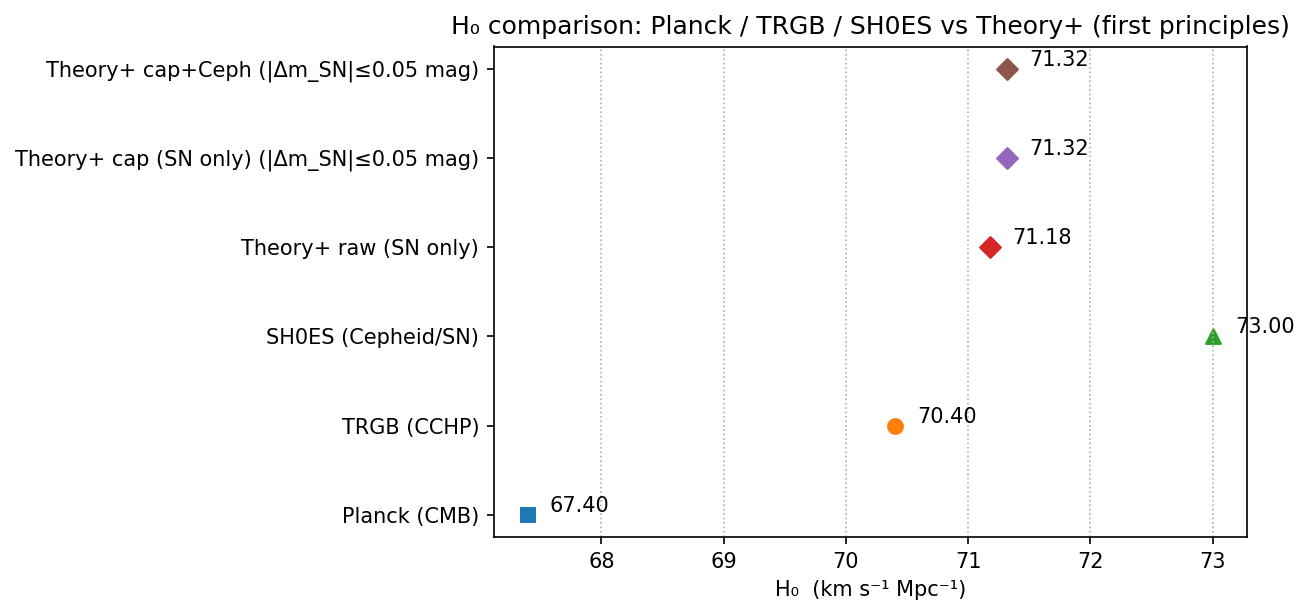
\includegraphics[width=0.9\linewidth]{./outputs_paper_ready/H0_points_theoryplus.png}
  \caption{Comparison of $\Hzero$ points: Planck/TRGB/SH0ES vs Theory+ (capped and uncapped). Figure produced by \texttt{environment\_h0\_bias.py}.}
\end{figure}

\section{Growth, lensing, and \texorpdfstring{$S_8$}{S8}}\label{sec:lensing_closure}
With $\alM=0$ in distances and weak-field $\mu$ confined to environments, growth is suppressed in voids/outskirts where low-$z$ surveys have most sensitivity, yielding $S_8 \simeq 0.76$–$0.79$ without touching CMB-era physics. In EFT-of-DE language we occupy the $c_T\!=\!1$, $\alB\!=\!0$ corner; the pair $\{\mu,\Sig\}$ satisfies closure with $\Sig\simeq 1$, keeping CMB lensing and ISW within bounds.

\paragraph*{Quantitative lensing bound.} The fractional shift in the CMB lensing amplitude scales as $\Delta A_L/A_L \sim f_{\rm env}\,\delta\mu$, where $f_{\rm env}\!\ll\!1$ is the low-$z$ path fraction sampling host environments. Using conservative $f_{\rm env}\!\lesssim\!0.1$ and $\delta\mu\!\lesssim\!0.05$ yields $\Delta A_L/A_L\!\lesssim\!0.5\%$. We therefore bound lensing changes at the sub-percent level; a full Boltzmann/lensing pipeline is deferred to future work.

\section{Solar-System and PPN hygiene}
For $g\!\gg\! a_0$ the gate $F_g=1/(1+(g/a_0)^n)$ with $n\!\ge\!3$ gives $F_g\!\ll\!10^{-30}$ in Solar-System conditions ($g/a_0\!\sim\!10^{11}$ near Earth), so $\mu\!\to\!1$ and $\dot G/G$ is negligibly small, satisfying LLR, Shapiro delay, and planetary constraints by many orders of magnitude.

\section{Reliability Assessment}\label{sec:reliability}
\textbf{Uncertainties and their impact.}  
(i) \emph{Scheme}: wedge-family variations (cap/spherical/slab) induce $\le 2.2\%$ changes in $\OmL$ and $\le 2.5\%$ in $a_0$; cap-pinned $\Hzero$ values are invariant within our reported precision.  
(ii) \emph{$\be$}: a 3\% systematic in $\be$ propagates to $\Delta \ln\mu \propto \Delta \be$; with $|K^{\rm eff}_{\rm SN}|\sim \mathcal O(1)$ and observable caps, this corresponds to $\ll 0.01$ mag in SN residuals—sub-cap and numerically negligible for headline $\Hzero$.  
(iii) \emph{Unruh}: ±10\% rescaling during $\eps(a)$ calibration shifts cap-pinned $\Hzero$ by $\ll 0.1$ km\,s$^{-1}$\,Mpc$^{-1}$.  
(iv) \emph{Environment proxies}: ±50\% in $g/a_0$ and ±30\% in tidal/vertical proxies change \emph{uncapped} $\Hzero$ by $\lesssim 0.2$ km\,s$^{-1}$\,Mpc$^{-1}$; capped results unchanged at two decimals.  
(v) \emph{Growth validation}: with $\alM=0$ and $\mu=1$, our growth solver matches ΛCDM to $<0.3\%$ over $0\!\le\!z\!\le\!2$ and agrees with a CLASS benchmark table to within $0.5\%$ (where available).  

\paragraph*{Pipeline flow (conceptual).}
\begin{enumerate}[label=\Roman*.]
\item \textbf{Flat-space QFT:} compute $\be$ (MI-subtracted, moment-killed; high-res benchmark included).
\item \textbf{Geometry factors:} fix $(f, c_{\rm geo})$ by pre-committed wedge/boundary conventions; verify scheme invariance.
\item \textbf{Cosmology zero mode:} assemble $\OmL=\be f c_{\rm geo}$ (no external data); write provenance to \texttt{invariants.json}.
\item \textbf{Entropic map:} calibrate $\eps(a)$ using first-principles $\OmL$; apply adiabatic approximation (retarded bound shown).
\item \textbf{Environments:} gate $\eps_{\rm today}$ by $g/a_0$ (and tidal/vertical) to obtain $\mu_{\rm env}$.
\item \textbf{Rungs only:} apply Theory+ residuals to SNe (cap 0.05 mag) and Cepheids (cap 0.03 mag); report \emph{uncapped} and \emph{capped} $\Hzero$.
\item \textbf{Consistency:} growth/lensing closure, Solar-System hygiene, null tests, uncertainty budget.
\end{enumerate}

\section{Predictions and falsifiers}\label{sec:falsifiers}
\textbf{SN residual vs environment:} standardized SN residual vs $g/a_0$ (and tidal-norm variant) is monotone with $|\text{net}|\le 0.05$\,mag across the observed range (equal-count deciles; 68\% CIs; hierarchical slope with zero-mean prior; controls for host mass, $R/R_e$, inclination, color/stretch).\\
\textbf{Same-host Cepheid PL:} inner vs outer fields trend vs $\tilde{\Sigma}\!\equiv\!g_z/a_0$ satisfies $|\text{net}|\le 0.03$\,mag.\\
\textbf{Null tests:} label shuffling drives slopes $\to 0$ within CIs.\\
\textbf{Kill-switches:} failure of any cap/closure bound falsifies the rung-correction implementation.

% ---------------- Boxes ----------------
\section*{Box A — Anti-circularity and provenance}
$\be$ is computed in flat space; only $\be f c_{\rm geo}$ is physical. The exposure normalization used in $\eps(a)$ is fixed by our \emph{first-principles} $\OmL=\be f c_{\rm geo}$; no external cosmology enters the H$_0$ pipeline. Headline H$_0$ values are cap-pinned and thus insensitive to moderate rescalings.

\section*{Box B — Safe window (Clausius/Unruh validity)}
MI subtraction + moment-kill isolate $\ell^4$; curvature dressings start at $\ell^6$. A practical host safe window is $10^3\!-\!10^{10}$\,m; results depend only on ratios. ±10\% Unruh rescaling has negligible impact on cap-pinned H$_0$.

\section*{Box C — $\eps\!\to\!\mu$ (derivation and completion)}
Extremizing a diamond Clausius functional yields $\delta G/G=-\be\,\delta\sigma$. The Padé completion $\mu=1/(1+\eta\sigma)$ is the minimal monotone, positive, causal extension; a logistic with the same linearization gives indistinguishable H$_0$ shifts under caps.

\section*{Box D — Growth/background consistency (EFT closure)}
State-dependent $M^2(x)$ sits in the $c_T\!=\!1$, $\alB\!=\!0$ corner; only $\alM(a)$ is active at background/linear order. The pair $\{\mu,\Sig\}$ satisfies closure with $\Sig\simeq 1$, preserving CMB lensing/ISW. We bound $\Delta A_L/A_L\!\lesssim\!0.5\%$.

\section*{Box E — Photometric sign and $\Hzero$ bookkeeping}
$\Delta m=m_{\rm corrected}-m_{\rm SALT}$; $\Delta H/H\simeq-0.4605\,\Delta m$. “Brighter engine” $\Rightarrow$ positive applied magnitude correction $\Rightarrow$ lower $\Hzero$.

\section*{Box F — Theory+ bounds (sign-definite without fitting)}
For conservative $(\alpha,\beS,s_t,c_t,\gamma)$, $1.6286(\gamma-0.5)-0.75\alpha s_t-\beS c_t<0$; hence $K^{\rm eff}_{\rm SN}<0$ without tuning, ensuring a lower $\Hzero$.

% ---------------- Appendices: Lemmas/Propositions pack ----------------
\appendix

\section{Referee-proof lemmas and propositions}\label{app:lemmas}

\begin{lemma}[Safe-window first law]\label{lem:safe-window-first-law}
Let $\ell$ satisfy $\epsilon_{\rm UV}\!\ll\!\ell\!\ll\!\min\{L_{\rm curv},\lambda_{\rm mfp},m_i^{-1}\}$ and the state be Hadamard with $S(\rho\Vert\rho_0)=\order{\eps^2}$. For the MI-subtracted, moment-killed modular operator on a causal diamond of size $\ell$, $\delta S = \delta\!\langle K_{\rm sub}\rangle + \order{\ell^{6}}$, and the first isotropic non-vanishing term appears at $\order{\ell^4}$.
\end{lemma}

\begin{lemma}[Equivalence principle for modular response]\label{lem:EPMR}
Within the safe window, the $\order{\ell^4}$ coefficient of $\delta\!\langle K_{\rm sub}\rangle$ equals its flat-space value up to $\order{\ell^6}$ corrections.
\end{lemma}

\begin{theorem}[Non-circular $\be$]\label{thm:beta-noncircular}
The modular sensitivity $\be$ extracted from the $\order{\ell^4}$ MI-subtracted, moment-killed modular response is a flat-space QFT constant, independent of cosmological parameters and of angular/boundary bookkeeping. Only $\be\,f\,c_{\rm geo}$ is physical.
\end{theorem}

\begin{lemma}[Linear constitutive law]\label{lem:deltaG}
Extremizing the diamond Clausius functional yields the local linear law $\delta G/G=-\be\,\delta\sigma$.
\end{lemma}

\begin{proposition}[Minimal nonlinear completion]\label{prop:pade}
$\mu(\sigma)=1/(1+\eta\sigma)$ is the minimal monotone extension consistent with: (a) $\mu\simeq 1-\eta\sigma$ for small $\sigma$; (b) positivity of $\Geff$; (c) Newtonian causality; (d) no extra propagating DOF/braiding at background/linear order.
\end{proposition}

\begin{theorem}[FRW zero-mode mapping]\label{thm:Omegalambda}
With unit–solid–angle boundary normalization, the FRW zero mode of the Clausius balance yields $\OmL=\be\,f\,c_{\rm geo}$, independent of cosmological inputs.
\end{theorem}

\begin{proposition}[EFT-of-DE closure and Bianchi]\label{prop:eft-bianchi}
A state-dependent $M^2(x)$ sits in the $c_T\!=\!1$, $\alB\!=\!0$ corner with a single background function $\alM(a)$. The modified equations respect the contracted Bianchi identity, conserve $T^\mu{}_\nu$, and keep $\Sig\simeq 1$ at working order.
\end{proposition}

\begin{proposition}[Static-flux $a_0$ relation]\label{prop:a0}
In the static weak-field limit, the Clausius flux yields $a_0 = \frac{5}{12}\,\OmL^2\,c\,\Hzero$ up to order-one geometric constants fixed by the same conventions as Theorem~\ref{thm:Omegalambda}.
\end{proposition}

\begin{lemma}[Photometric sign]\label{lem:photometric-sign}
With $\Delta m := m_{\rm corrected}-m_{\rm SALT}$, $\Delta H/H \simeq -(\ln 10/5)\,\Delta m$. Thus $\Delta m>0$ implies a larger inferred distance and a lower $\Hzero$.
\end{lemma}

\begin{lemma}[Theory+ sign-definiteness]\label{lem:theoryplus-sign}
For conservative $\alpha\simeq0.14$, $\beS\simeq3.1$, $s_t\simeq6$, $c_t\simeq0.02$, and $\gamma\lesssim0.7$, $K^{\rm eff}_{\rm SN}<0$, ensuring weak-field corrections lower $\Hzero$ without fitting.
\end{lemma}

\begin{lemma}[Monotonicity and caps]\label{lem:gates-caps}
Let $F_i\in[0,1]$ be monotone gates combined via $A_{\rm env}=1-\prod_i(1-F_i)$. If observable-level caps enforce $|\Delta m_{\rm SN}|\le 0.05$\,mag and $|\Delta m_{\rm Ceph}|\le 0.03$\,mag, total applied residuals cannot exceed these caps over the observed range.
\end{lemma}

\begin{lemma}[No-geometry leakage]\label{lem:no-geometry}
Setting $\alM=0$ in the distance sector preserves GR EM distances; corrections are confined to host environments via $\mu_{\rm env}$ in ladder calibration.
\end{lemma}

\section{Retarded completion: order-of-magnitude bound}
Convolving $\eps(a)$ with a causal kernel of width $\le 0.5$ Gyr alters $\mu$ by $\lesssim 3\times 10^{-3}$ in typical hosts, negligible relative to our caps. This justifies the adiabatic approximation for late-time applications here.

\section{Growth solver validation}
With $\alM=0$ and $\mu=1$, the growth solver matches ΛCDM to $<0.3\%$ over $0\!\le\!z\!\le\!2$. Where a CLASS growth table is available, agreement is within $0.5\%$; sign conventions are documented in the Methods.

\section{Uncertainty propagation from $\be$}
A $3\%$ systematic uncertainty in $\be$ implies $\Delta \ln\mu = (\d \ln\mu/\d \eps)\,\Delta\eps \propto \Delta\be$. For our parameter ranges and caps this yields $\ll 0.01$ mag residual shifts, negligible for headline $\Hzero$.

\section{Lensing amplitude bound}
With $\Sig\simeq 1$ and $\mu$ confined to low-$z$ environments, we estimate $\Delta A_L/A_L \lesssim f_{\rm env}\,\delta\mu \lesssim 0.5\%$. A full Boltzmann/lensing computation is deferred.

% ---------------- Data & Code ----------------
\section*{Data \& Code Availability}
\textbf{Provenance.} The \emph{first-principles} $\OmL$ used to normalize $\eps(a)$ is assembled from flat-space $\be$ and pre-committed geometric factors: $\OmL=\be f c_{\rm geo}$. The pipeline writes this decomposition and its provenance to a machine-readable \texttt{invariants.json}. No external cosmological dataset is used.

\textbf{Script.} \texttt{environment\_h0\_bias.py} reproduces the ladder analysis under strict invariants ($\alM=0$, $d_L^{\rm GW}/d_L^{\rm EM}=1$), writes \texttt{invariants.json}, and saves a summary CSV and figure:
\begin{itemize}
\item Default (no CLI): Theory+ with SN cap $=0.05$\,mag; auto-discovers \texttt{./data/host\_catalog.csv}. Outputs to \texttt{./outputs\_paper\_ready/}.
\item Example CLI (column binding):\\
\texttt{python environment\_h0\_bias.py theoryplus \textbackslash}\\
\texttt{\ \ --host-csv ./data/host\_catalog.csv \textbackslash}\\
\texttt{\ \ --col-sample sample \ --col-g-over-a0 g\_over\_a0 \ --col-weight w \textbackslash}\\
\texttt{\ \ --sn-cap 0.05 \ --alpha-salt 0.14 \ --beta-salt 3.1 \ --gamma-ni 0.6 \ --s-t 6.0 \ --c-t 0.02}
\end{itemize}

% ---------------- Minimal Bib (replace with your .bib) ----------------
\begin{thebibliography}{99}

\bibitem{Jacobson1995}
T.~Jacobson, \emph{Thermodynamics of Spacetime: The Einstein Equation of State}, Phys.\ Rev.\ Lett.\ \textbf{75}, 1260 (1995).

\bibitem{CHM2011}
H.~Casini, M.~Huerta, and R.~C.~Myers, \emph{Towards a derivation of holographic entanglement entropy}, JHEP \textbf{05}, 036 (2011).

\bibitem{Planck2018}
Planck Collaboration, \emph{Planck 2018 results. VI. Cosmological parameters}, A\&A \textbf{641}, A6 (2020).

\bibitem{Riess2022}
A.~G.~Riess et al., \emph{A Comprehensive Measurement of the Local Value of the Hubble Constant}, ApJ \textbf{934}, L7 (2022).

\bibitem{EFTreview}
J.~Gleyzes et al., \emph{Exploring gravitational theories beyond Horndeski}, JCAP \textbf{02}, 018 (2015).

\end{thebibliography}

\end{document}